%!TEX program = xelatex 
\documentclass[a4paper,zihao=-4]{article}
\usepackage[UTF8,punct,linespread=1.56]{ctex}
% \documentclass[a4paper,cs4size,UTF8,punct,linespread=1.56]{ctexart}
\pagestyle{empty} % 第二页以后页码空白
\usepackage[a4paper, left = 3.2cm, right = 3.2cm, top = 2.54cm, bottom = 2.54cm]{geometry}
\usepackage{xcolor}
% \usepackage[citebordercolor = white]{hyperref}
\usepackage[hidelinks]{hyperref}
\usepackage{graphicx} 
\usepackage{amsmath}
\usepackage{amssymb}
\usepackage{times}
\usepackage{multirow}
\usepackage[subrefformat=parens,labelformat=parens]{subfig} %
\usepackage{booktabs} % for \toprule \midrule \bottomrule \cmidrule
\usepackage{cleveref}
\crefformat{table}{表~#2#1#3 }
\crefformat{figure}{图~#2#1#3 }
\crefformat{equation}{式~(#2#1#3)}
\crefformat{chapter}{#2第#1章#3}
\crefformat{section}{#2第#1节#3}
\crefformat{subsection}{#2第#1节#3}
\crefformat{subsubsection}{#2第#1节#3}

\usepackage{tikz}
\usetikzlibrary{backgrounds,mindmap,calc,positioning,intersections}
\tikzstyle{startstop} = [rectangle, rounded corners, minimum width = 1cm, minimum height=0.5cm,text centered, draw = black]
\tikzstyle{io} = [trapezium, trapezium left angle=70, trapezium right angle=110, minimum width=1cm, minimum height=0.5cm, text centered, draw=black]
\tikzstyle{process} = [rectangle, minimum width=3cm, minimum height=1cm, text centered, draw=black]
\tikzstyle{decision} = [diamond, aspect = 3, text centered, draw=black]
% 箭头形式
\tikzstyle{arrow} = [->,>=stealth]

\usepackage{enumitem}
% \setenumerate[1]{itemsep = 0pt, parsep = 0pt, topsep = 2bp}
\setlist[enumerate]{itemsep = 0pt, parsep = 0pt, topsep = 2bp}
% \setitemize[1]{itemsep = 0pt, parsep = 0pt, topsep = 2bp}
\setlist[itemize]{itemsep = 0pt, parsep = 0pt, topsep = 2bp}
\usepackage{fontspec}
\setmainfont{Times New Roman}
% \usepackage{minted}   % For syntax highlighting
% \usemintedstyle{friendly}
\usepackage{setspace} 
\usepackage{caption}
\DeclareCaptionFont{capfont}{\kaishu\zihao{-4}\selectfont} % Caption font
\DeclareCaptionFont{subfont}{\kaishu\zihao{5}\selectfont} % Sub-caption font
\captionsetup{font = capfont}
\captionsetup[subfigure]{font = subfont}
\captionsetup[figure]{labelsep=space} % 空格 space;点 period;冒号 colon
\captionsetup[table]{labelsep=space}  % 空格 space;点 period;冒号 colon
\usepackage[square,numbers,sort&compress]{natbib}   % For Reference
\newcommand{\citess}[1]{\textsuperscript{\cite{#1}}}
\setlength{\bibsep}{1pt plus 0.3ex}
\usepackage{titlesec}
\titleformat{\subsubsection}[block]{\hspace{3em}}{\thesubsubsection}{1em}{}
\usepackage{insfc}



\graphicspath{{images/}}   % 设置图片所存放的目录

\begin{document}

\songti
%\kaishu

% Decrease space above and below equations
\setlength{\abovedisplayskip}{0pt}
\setlength{\belowdisplayskip}{0pt}

%%%%%%%%% TITLE %%%%%%%%%
% \title{报告正文 \vspace{-3.4ex}}
% \title{报告正文}
% \maketitle
\begin{center}
	{\kaishu \zihao{3} \textbf{报告正文} \vspace{-3ex}}
\end{center}  

\thispagestyle{empty}    % 首页页码空白


{\kaishu \zihao{4}参照以下提纲撰写,要求内容翔实、清晰,层次分明,标题突出。}\alert{请勿删除或改动下述提纲标题及括号中的文字。\vspace{9bp}}

\NsfcChapter{(一)立项依据与研究内容}{\kaishu(建议8000字以内):}

\NsfcSection{1}{项目的立项依据}{(研究意义、国内外研究现状及发展动态分析,需结合科学研究发展趋势来论述科学意义;或结合国民经济和社会发展中迫切需要解决的关键科技问题来论述其应用前景。附主要参考文献目录);}

\subsection{研究背景和意义}
与中微子振荡相关的物理现象揭示了超出标准模型的新物理,是当前的研究热点。在目前三代中微子混合框架下,决定中微子振荡的参数包含两个质量平方差$\Delta m_{21}^2$和$\Delta m_{32}^2$,三个混合角$\theta_{12}$、$\theta_{23}$和$\theta_{13}$,以及CP破坏相角$\delta_{\text{CP}}$。其中,$\Delta m_{32}^2$的符号、$\theta_{23}$的卦限和$\delta_{\text{CP}}$都是尚未知的。如果$\theta_{13}$为0,由于其与$\delta_{\text{CP}}$的耦合关系,将无法通过振荡现象研究轻子CP破坏。2012年,大亚湾反应堆中微子实验\citess{DayaBay:2012fng}首次以超过五倍标准偏差的显著度测量出$\theta_{13}$不为0。而且,测量出的$\theta_{13}$值比预期的要大,使得通过中微子振荡现象确定$\delta_{\text{CP}}$成为可能。此后,大亚湾实验一直提供了国际上最精确的$\theta_{13}$测量结果。\qiangdiao{当下,继续利用大亚湾实验未使用的大统计量数据提高$\theta_{13}$的测量精度,对于探索这些中微子物理的未知量:$\Delta m_{32}^2$的符号、$\theta_{23}$的卦限与$\delta_{\text{CP}}$将起到关键作用。}

\paragraph{\qiangdiao{\textbf{CP破坏相角与$\mathbf{\theta_{13}}$。}}}CP对称性破缺在1964年被首次提出\citess{Christenson:1964fg}。它被认为是解释宇宙中正反物质不平衡现象的必要条件\citess{Sakharov:1967dj}。而中微子被认为是很可能揭开CP破坏起源之谜的粒子。目前,对轻子中的$\delta_{\text{CP}}$最好的限制结果来自日本的T2K实验\citess{T2K:2021xwb}和美国的NOvA实验\citess{NOvA:2021nfi}。他们的研究基于加速器中微子束流中的$\nu_\mu\to\nu_e$和$\overline{\nu}_\mu\to\overline{\nu}_e$振荡现象开展。T2K实验给出的最新结果是$\delta_{\text{CP}}$的值在最大CP破坏对应的$\pi/2$附近,$\delta_{\text{CP}}=0$和$\delta_{\text{CP}}=\pi$都在95\%的置信度下被排除。\qiangdiao{从\cref{tab:CP-measurements}进一步看出,使用反应堆中微子实验提供的$\theta_{13}$精确测量结果,能大大提升T2K实验对$\delta_{\text{CP}}$的限制精度。NOvA实验则直接使用了反应堆中微子实验的$\theta_{13}$测量结果,但其研究却受到$\theta_{23}$卦限假设的影响。}在给定质量次序和$\theta_{23}$卦限假设下,NOvA实验得到的90\%置信水平下的$\delta_{\text{CP}}$范围覆盖了所有可能的值,并未给出CP破坏存在与否的倾向。在未来实验中,更高的$\theta_{13}$精度和明确的$\theta_{23}$卦限对$\delta_{\text{CP}}$范围的进一步确定具有重要意义。
\begin{table}[htb!]
	\centering
	\setlength{\tabcolsep}{10pt}
	\zihao{5}
	\caption{T2K\citess{T2K:2021xwb}和NOvA\citess{NOvA:2021nfi}实验对$\delta_{\text{CP}}$最新的限制结果和一倍标准偏差。其中,NO为正质量次序假设,IO为反质量次序假设。T2K only代表T2K实验不使用反应堆中微子实验对$\theta_{13}$的测量结果,T2K+Reactor则代表T2K实验使用反应堆中微子实验对$\theta_{13}$的测量结果来提升显著度。UO和LO代表$\theta_{23}$的不同卦限,分别对应于$\theta_{23}>45^\circ$和$\theta_{23}<45^\circ$.}
	\begin{tabular}{ccccc}
		\toprule
		\multirow{2}{*}{质量次序假设} & \multicolumn{2}{c}{T2K实验} & \multicolumn{2}{c}{NOvA实验} \\ 
		\cmidrule{2-3} \cmidrule{4-5}
	& \multicolumn{1}{c}{T2K only} & \multicolumn{1}{c}{T2K+Reactor} & \multicolumn{1}{c}{UO} & \multicolumn{1}{c}{LO} \\
		\midrule          
		NO & $-2.14^{+0.90}_{-0.69}$ & $-1.89^{+0.70}_{-0.58}$ & $2.58^{+0.85}_{-2.73}$ & $0.22^{+0.94}_{-0.82}$ \\
		IO & $-1.26^{+0.61}_{-0.69}$ & $-1.38^{+0.48}_{-0.55}$ & $4.78^{+0.85}_{-0.94}$ & $4.43^{+0.57}_{-0.69}$ \\
		\bottomrule
	\end{tabular}%
	\label{tab:CP-measurements}%
\end{table}%

\paragraph{\qiangdiao{\textbf{$\mathbf{\theta_{23}}$的卦限与$\mathbf{\theta_{13}}$。}}}对$\theta_{23}$的测量主要是通过加速器中微子和大气中微子实验中$\nu_\mu\to\nu_\mu$和$\overline{\nu}_\mu\to\overline{\nu}_\mu$的振荡现象开展的。对这两个振荡通道观测可以测量出$2\theta_{23}$接近于$90^\circ$,但无法确定$2\theta_{23}>90^\circ$还是$<90^\circ$。通过加速器和大气中微子实验中的$\nu_\mu\to\nu_e$和$\overline{\nu}_\mu\to\overline{\nu}_e$的振荡可以确定$\theta_{23}$卦限\citess{Agarwalla:2013ju}。该振荡通道的主要几率项的振幅与$\sin^22\theta_{13}$成正比。\qiangdiao{因此,$\theta_{13}$的精度提升将直接降低观测该振荡现象的不确定度,帮助$\theta_{23}$参数的确定。}

\paragraph{\qiangdiao{\textbf{中微子质量次序与$\mathbf{\theta_{13}}$。}}}中微子质量次序的确定是粒子物理学和宇宙学的主要挑战之一,这不仅因为它能影响自然界质量产生的基本理论,而且能决定未来无中微子双$\beta$衰变实验的规模\citess{Gariazzo:2022ahe}。目前大部分实验结果和国际上的联合分析\citess{Esteban:2020cvm,Kelly:2020fkv}结果显示,数据更倾向于支持正质量次序(NO)而非反质量次序(IO),但也未排除联合分析可能会支持IO假设的可能性。目前,对中微子质量次序敏感的实验结果主要来自T2K实验\citess{T2K:2021xwb},NOvA实验\citess{NOvA:2021nfi},MINOS实验\citess{2018npa..confE.423A},Super-K实验\citess{Super-Kamiokande:2017yvm}和IceCube/DeepCore实验\citess{IceCube:2017lak}。未来的JUNO\citess{JUNO:2021vlw},Hyper-K\citess{Hyper-Kamiokande:2022smq}和DUNE\citess{DUNE:2020fgq}等实验都将提升对中微子质量次序的灵敏度。中微子质量次序可以通过GeV能量以上的大气中微子及其天顶角依赖性来确定。物质效应对振荡概率的影响可以使$\nu_\mu\to\nu_e$的振荡在NO假设下增强,而使$\overline{\nu}_\mu\to\overline{\nu}_e$的振荡在IO假设下增强。加速器实验也可以基于相同的效应探索中微子的质量次序。比如,这一效应可以使NOvA实验观测到的振荡概率改变约20\%\citess{NOvA:2021nfi}。\qiangdiao{与$\theta_{23}$卦限的确定类似,$\nu_\mu\to\nu_e$和$\overline{\nu}_\mu\to\overline{\nu}_e$的振荡概率主要项都与$\theta_{13}$有关。$\theta_{13}$精度的提升对这些中微子物理未知参数的确定都具有重要意义。}

\subsection{国内外研究现状及分析}
国际上对$\theta_{13}$灵敏度最高的实验主要是短基线反应堆中微子实验,包括中国的大亚湾实验\citess{DayaBay:2022orm},韩国的RENO实验\citess{RENO:2018dro}和法国的Double Chooz实验\citess{DoubleChooz:2019qbj}。2012年,大亚湾实验\citess{DayaBay:2012fng}首次以超过五倍标准偏差的显著度测量出$\theta_{13}$不为0,发现了新的中微子振荡模式,之后被RENO实验\citess{RENO:2012mkc}和Double Chooz实验\citess{DoubleChooz:2012gmf}确认。

大亚湾实验于2011年12月24日开始采数,2020年12月12日停止采数。RENO实验于2011年8月11日开始采数,目前仍在运行。Double Chooz实验于2015年1月开始以多个探测器开始运行采数,2017年12月份停止采数。

大亚湾实验在整个运行时期内在三个实验厅(EH1,EH2和EH3)前后共安装有八个全同设计的探测器,用于探测大亚湾、岭澳一期和岭澳二期共六个核电反应堆释放出的反电子中微子 ($\overline{\nu}_e$)。\qiangdiao{由于采用多个探测器进行相对测量,大亚湾实验可以大大降低反应堆、探测效率等探测器间关联的不确定因素的干扰,获得比以往实验明显更高的灵敏度。}实验厅EH1的两个探测器(EH1-AD1和EH1-AD2)与大亚湾反应堆距离约360 m,EH2的两个探测器(EH2-AD1和EH2-AD2)与岭澳一期和岭澳二期反应堆相距约500 m。在这种距离下,反应堆释放出的$\overline{\nu}_e$的振荡效应极其微小,可以对反应堆中微子的流强进行精确测量。EH3的四个探测器(EH3-AD1,EH3-AD2,EH3-AD3和EH3-AD4)与大亚湾和岭澳反应堆的距离分别约为1.9 km和1.5 km。在这一飞行距离下,$\overline{\nu}_e$存活几率中与$\Delta m_{31}^2$/$\Delta m_{32}^2$相关的振荡项成为主导,其对应的振幅近似为$\sin^22\theta_{13}$,如\cref{eq:oscillation-prob}所示。
\begin{equation}\label{eq:oscillation-prob}
	\begin{aligned}
P_{\text {sur }}= & 1-\cos ^4 \theta_{13} \sin ^2 2 \theta_{12} \sin ^2 \Delta_{21} \\
& -\sin ^2 2 \theta_{13}\left(\cos ^2 \theta_{12} \sin ^2 \Delta_{31}+\sin ^2 \theta_{12} \sin ^2 \Delta_{32}\right),
\end{aligned}
\end{equation}
其中$\Delta_{j i} \simeq 1.267 \Delta m_{j i}^2\left(\mathrm{eV}^2\right) L(\mathrm{~m}) / E_\nu(\mathrm{MeV})$. 
当$\overline{\nu}_e$穿过探测器,有一定概率与其中的质子发生反$\beta$衰变反应(IBD)。如\cref{eq:IBD}所示,IBD反应末态会生成两个粒子:正电子和中子。
\begin{equation}\label{eq:IBD}
	\overline{\nu}_e+p\to e^++n
\end{equation}
正电子如果穿过探测器中心的掺钆液闪(GdLS)和中间的纯液闪(LS)区域,会很快地损失能量形成快信号。而中子则先被慢化,然后会被核俘获,俘获核继而释放出$\gamma$从而形成慢信号。在实验中,中子主要被钆核和氢核所俘获。在GdLS和LS区间对应的俘获时间分别约为30 $\mu$s和200 $\mu$s。因此,IBD信号的明显特征是正电子形成的快信号与中子俘获形成的慢信号在时间上的符合。中子被钆核俘获对应的IBD数据样本被称为钆俘获样本($n$Gd-IBD),该样本由钆核释放出的总能量约8 MeV的几个$\gamma$标记。由于该特征能量很高,$n$Gd分析受本底的影响很小。中子被氢核俘获对应的IBD数据样本被称为氢俘获样本($n$H-IBD),该样本由氢核释放出的单个2.2 MeV的$\gamma$标记。由于2.2 MeV附近存在很多放射性活动形成的本底,$n$H-IBD样本的研究受本底影响较大。比如在EH3中,$\overline{\nu}_e$信号数与本底数接近$1:1$。此外,$n$H-IBD信号主要来自中心钆俘获区域外侧的纯液闪,在该区域产生的粒子可能无法将全部的能量留在探测器中形成光信号从而产生能量泄露。\qiangdiao{这也使$n$H样本与$n$Gd样本相比,具有统计和系统上的明显独立性。}RENO和Double Chooz实验的基本策略与大亚湾实验类似,但测量精度更低,在此不再赘述。

由于$n$H分析的上述困难,大亚湾和RENO实验基于单一样本最精确的测量都由$n$Gd分析\citess{DayaBay:2022orm,RENO:2018dro}提供,精度分别为2.8\%和7.5\%。\qiangdiao{但这些实验都采用独立的$n$H样本来提供交叉检验\citess{DayaBay:2014fud, DayaBay:2016ziq, RENO:2019otc}}。Double Chooz实验受限于明显更低的统计量,其最精确的测量结果由全中子俘获样本的分析\citess{DoubleChooz:2019qbj}提供,精度为13\%。除了这三组实验外,加速器和大气中微子实验可以利用$\nu_\mu\to\nu_e$和$\overline{\nu}_\mu\to\overline{\nu}_e$的振荡对$\theta_{13}$进行测量,但其灵敏度远不如反应堆实验。如\cref{fig:world-status},展示了国际上各种实验提供的$\theta_{13}$和$\Delta m_{32}^2$测量结果。其中,黑色点展示的是大亚湾实验3158天的完整钆俘获样本测量结果\citess{DayaBay:2022orm},已提交到预印本网站\texttt{arxiv.org}上;红色点展示的是基于大亚湾实验1958天采集的氢俘获样本研究的测量结果,已完成合作组内部分析评审。
\begin{figure}[!htb]
    \centering
    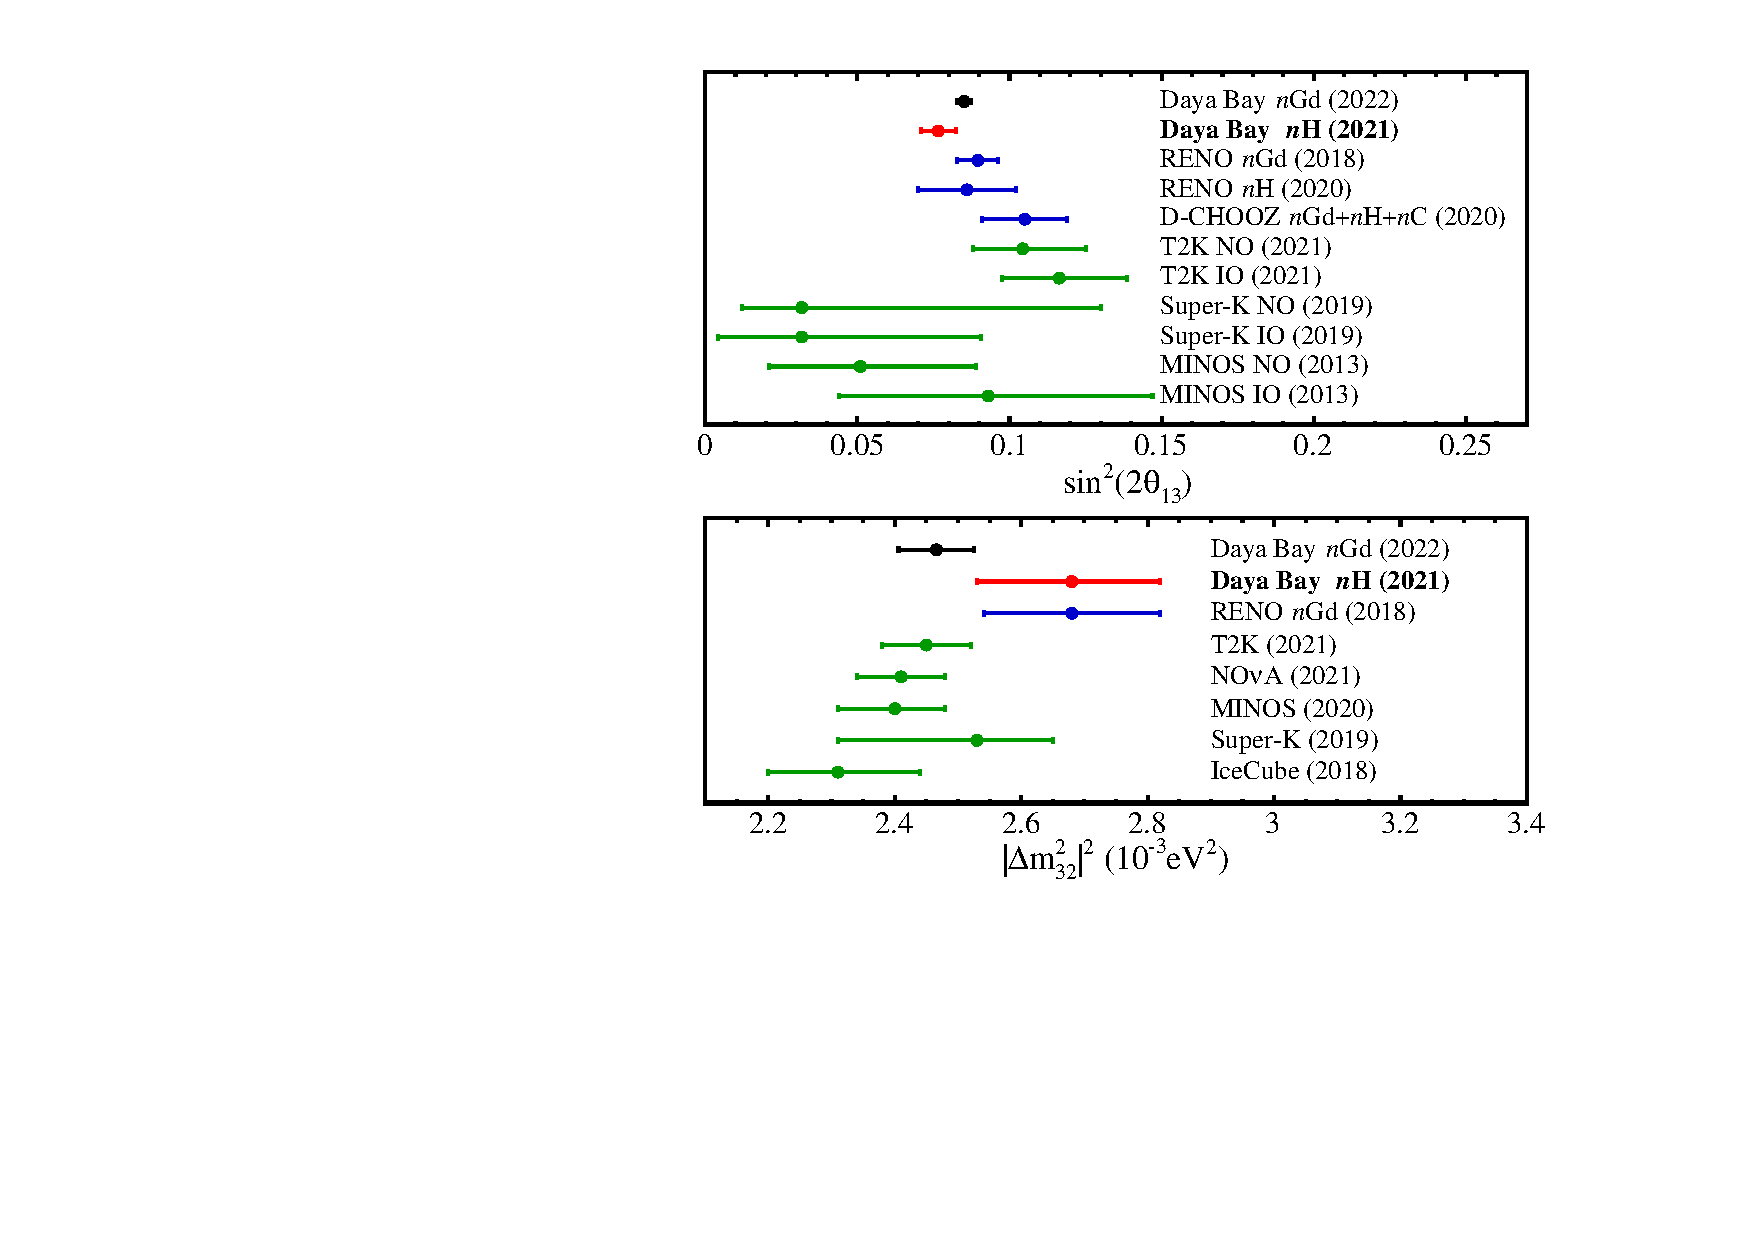
\includegraphics[width=15cm]{WorldMeas.pdf}
    \caption{世界上各种实验对$\sin^22\theta_{13}$(上图)和$\Delta m_{32}^2$(下图)的测量结果比较。其中黑点展示的是大亚湾实验$n$Gd分析的结果\citess{DayaBay:2022orm}(使用完整的3158天数据),红点展示的是大亚湾实验$n$H分析的结果(使用1958天数据),蓝点展示的是RENO和Double Chooz实验使用不同样本的测量结果\citess{RENO:2018dro,RENO:2019otc,DoubleChooz:2019qbj},绿点展示了加速器实验:T2K\citess{T2K:2021xwb},Super-K\citess{Super-Kamiokande:2019gzr},MINOS/MINOS+\citess{MINOS:2013xrl,MINOS:2020llm}和IceCube\citess{IceCube:2017lak}提供的测量结果。$\Delta m_{32}^2$测量值都是NO假设下的结果。IO假设下的比较与之类似,此处不再展示。}
    \label{fig:world-status}
\end{figure}

\subsection{项目研究动机}
大亚湾和RENO提供的最精确的$\sin^22\theta_{13}$测量结果都是来自$n$Gd分析。大亚湾实验目前最新发表的$n$H样本的$\theta_{13}$测量\citess{DayaBay:2016ziq}出自2016年,只使用了621天的数据。\qiangdiao{大亚湾实验新近完成合作组评审的$n$H分析使用的数据只占完整数据的约62\%,但其提供的$\sin^22\theta_{13}$的测量精度已经达到RENO最新的$n$Gd分析结果的精度。使用大亚湾完整数据集(与1958的数据相比,统计量提升约为60\%)开展此项$n$H研究,额外1200天数据的加入将给统计和系统误差都带来巨大改进。因此,基于大亚湾实验$n$H样本的$\theta_{13}$测量精度还有很大的提升空间。而且本项目将联合$n$H和$n$Gd分析的结果进一步改进精度。}

本项目旨在通过联合$n$H和$n$Gd分析的$\sin^22\theta_{13}$测量结果,给出国际上最精确的$\theta_{13}$测量值,同时$\Delta m_{32}^2$的测量精度也位于世界前列。目前,完整钆俘获数据集的研究已经完成,使用62\%的氢俘获数据集的工作也已完成。延续这些工作,本项目将完成下述物理目标:
\begin{enumerate}
	\item 使用完整氢俘获样本完成$\theta_{13}$测量。\qiangdiao{预期本项目将给出国际上第二精确的$\theta_{13}$测量结果,精度约6\%},并将此项结果对最终联合结果贡献的权重从之前的15\%提高到约20\%。
	\item 将完整氢俘获数据样本的研究结果与已公开的完整钆俘获数据样本的研究结果\citess{DayaBay:2022orm}进行联合,\qiangdiao{给出大亚湾实验最终的$\theta_{13}$测量结果,将其2.8\%的测量精度改进到约2.5\%}。
\end{enumerate}

\begin{spacing}{1.3} % 行距
	\zihao{5} \songti   
	\bibliographystyle{apsrev4-2}
	\bibliography{ref}  
	\vspace{11bp}
\end{spacing}

\NsfcSection{2}{项目的研究内容、研究目标,以及拟解决的关键科学问题}{(此部分为重点阐述内容);}
\subsection{研究内容}

本项目依托于大亚湾反应堆中微子实验,研究内容主要分为三个部分:1. $n$H样本的信号与本底分析;2. 系统误差分析与振荡参数拟合;3. $n$H和$n$Gd分析结果的联合。

\subsubsection{$n$H样本的信号与本底分析}\label{sec:backgrounds}
从大亚湾已经完成刻度与重建的数据出发,根据每个事例在时间上的关联性,使用一个固定时间窗,比如1500 $\mu$s,可以筛选出数据中的$\overline{\nu}_e$形成的快慢信号事例对。快信号的能量范围被要求为$[1.5, 12]$ MeV,以尽可能包含所有的中微子信号并排除1.5 MeV下的放射性关联本底,比如$^{214}\text{Bi}-^{214}\text{Po}$和$^{212}\text{Bi}-^{212}\text{Po}$形成的$\beta$-$\alpha$级联衰变本底。慢信号的能量则处于2.2 MeV附近,对应于中子被氢核俘获释放出$\gamma$的能量。进一步筛选快慢事例之间的距离和时间,比如距离小于500 mm和时间小于400 $\mu$s,可以得到信噪比增强的$\overline{\nu}_e$候选事例样本。根据目前的研究,该样本包含有五种本底:偶然符合本底、$^9$Li/$^8$He本底、快中子本底、muon-x本底、放射性中子本底和Am-C中子刻度源本底。

\paragraph{偶然符合本底}

偶然符合本底是单事例在时间窗内随机成对组合并满足筛选条件而形成的。这些单事例基本都来自探测器内部材料和外部环境的放射性活动。该本底的事例率可以通过距离筛选条件被压低两个数量级。

\paragraph{$^9$Li/$^8$He本底}宇宙线缪子及其散裂产物可以与有机液闪中的$^{12}$C发生强和电磁相互作用,产生中子和新的同位素。在这些宇生同位素中,$^9$Li 和 $^8$He 可以通过$\beta^-$衰变转变为一个不稳定的核素,然后立即释放出一个中子。这样的 $\beta$-$n$ 级联衰变就可以构成IBD信号的本底。$^9$Li 和 $^8$He 的寿命分别约为 257 ms 和 172 ms,这比实验中对绝大部分缪子的反符合时间都要长。而且它们的快信号 $\beta$ 的能量最高可以达到 13.6 MeV,与 IBD 事例的快信号能量有很大一部分重叠。
\paragraph{快中子本底}宇宙线缪子还可以生成高能的散裂中子。后者在进入到探测器的过程中被慢化,会留下反冲信号作为快信号,然后被俘获从而留下中子俘获的慢信号,形成IBD信号的本底。探测器外部水池对宇宙线缪子具有很高的标记效率,并且对在探测器中留下能量的缪子反符合时间较长,因此在探测器内部形成的快中子基本无法被筛选进信号样本中。但宇宙线缪子在水池外部的岩石中形成的快中子却可以逃过反符合系统。从外部而来的快中子形成的本底事例更多地集中在 LS 区域,因而该本底对$n$H分析的影响比对$n$Gd分析更大。
\paragraph{\qiangdiao{muon-x本底}}\qiangdiao{实验末期,由于水池顶部附近PMT的性能逐渐下降,外水池的宇宙线缪子反符合效率随时间下降。一些低能的缪子可以穿过水池而不被探测到。缪子形成的快信号,与缪子衰变产生的Michel电子或者散裂中子形成的慢信号一起构成了IBD信号的本底。}
\paragraph{放射性中子本底}
放射性中子主要是通过核素自裂变和$(\alpha,n)$反应产生的。这两个过程在产生中子的同时,还会产生伴随的$\gamma$。这些中子和$\gamma$有一定概率进入到中心的液闪区域并沉积能量。中子的反冲信号和$\gamma$可以形成快信号,中子俘获则可形成慢信号,这样就构成了IBD信号的本底。核素的每次自发裂变一般会同时产生多个$\gamma$和中子,因此除了以$(\alpha,n)$类似的机制形成本底外,还可以通过多个中子俘获之间的符合形成本底。

此外,还有自动刻度源中的Am-C中子源形成的核反冲与中子俘获在时间上的关联快慢信号,也可形成IBD信号的本底,是$n$H样本本底中占比最少的一项。

根据已经完成的1958天数据的分析,近点探测器观测到的IBD信号占总的$\overline{\nu}_e$候选样本的约88\%,具有较好的信噪比。远点探测器观测到的IBD信号占总的$\overline{\nu}_e$候选样本的约50\%。而除偶然符合本底以外的关联本底只占总样本的约0.6\%,其中muon-x本底在$n$H样本中的分析将在本项目中首次开展。\cref{fig:nH-nGd-bkgs}展示了1958天数据分析中,远厅EH3的$n$H和$n$Gd样本的本底与信号叠加能谱。$n$H样本在3 MeV以下较高的本底水平明显可见,而$n$Gd样本在整个能谱都有较好的信噪比。

\begin{figure}[!htb]
    \begin{minipage}[t]{0.5\linewidth}
    \centering
        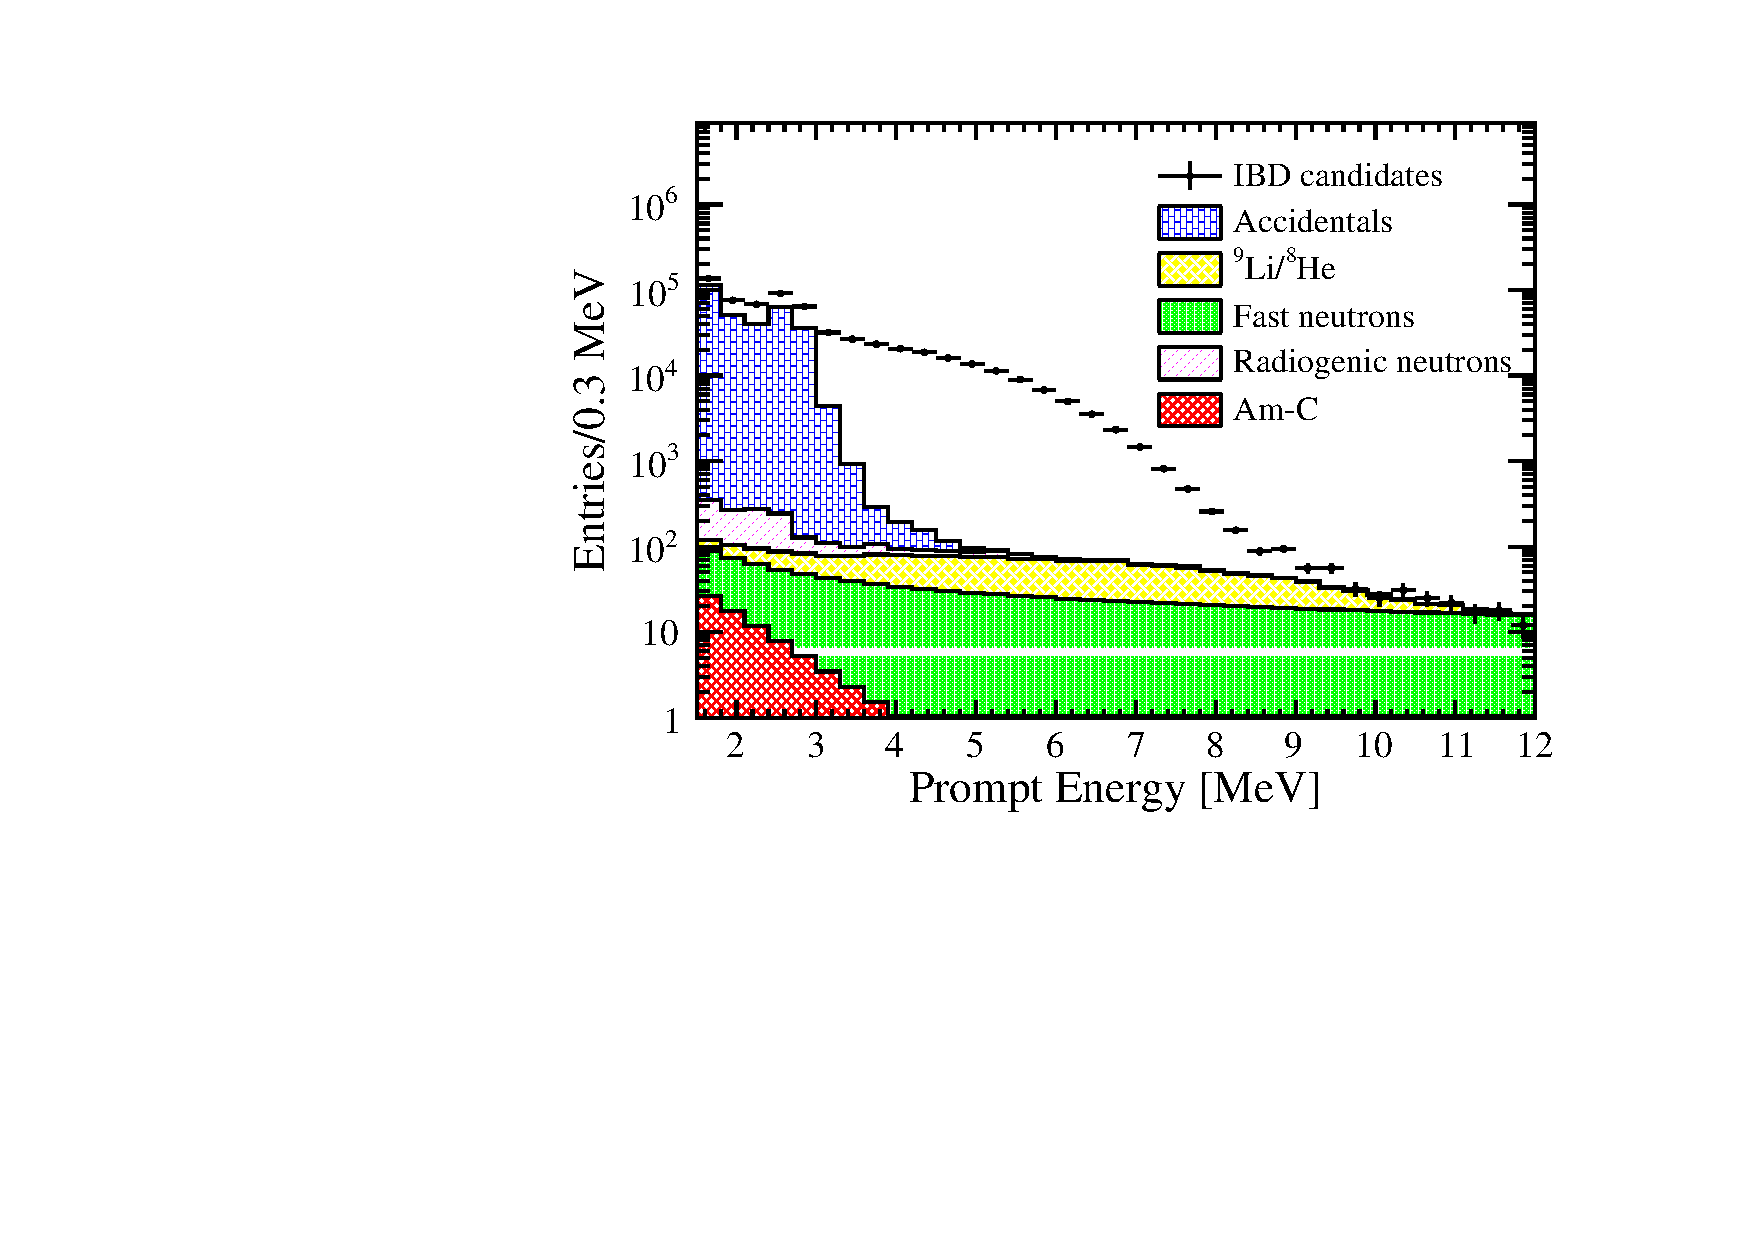
\includegraphics[width=8cm]{spec_stack_EH3_best.pdf}
    \caption*{(a)}
    \end{minipage}
    \begin{minipage}[t]{0.5\linewidth}
    \centering
        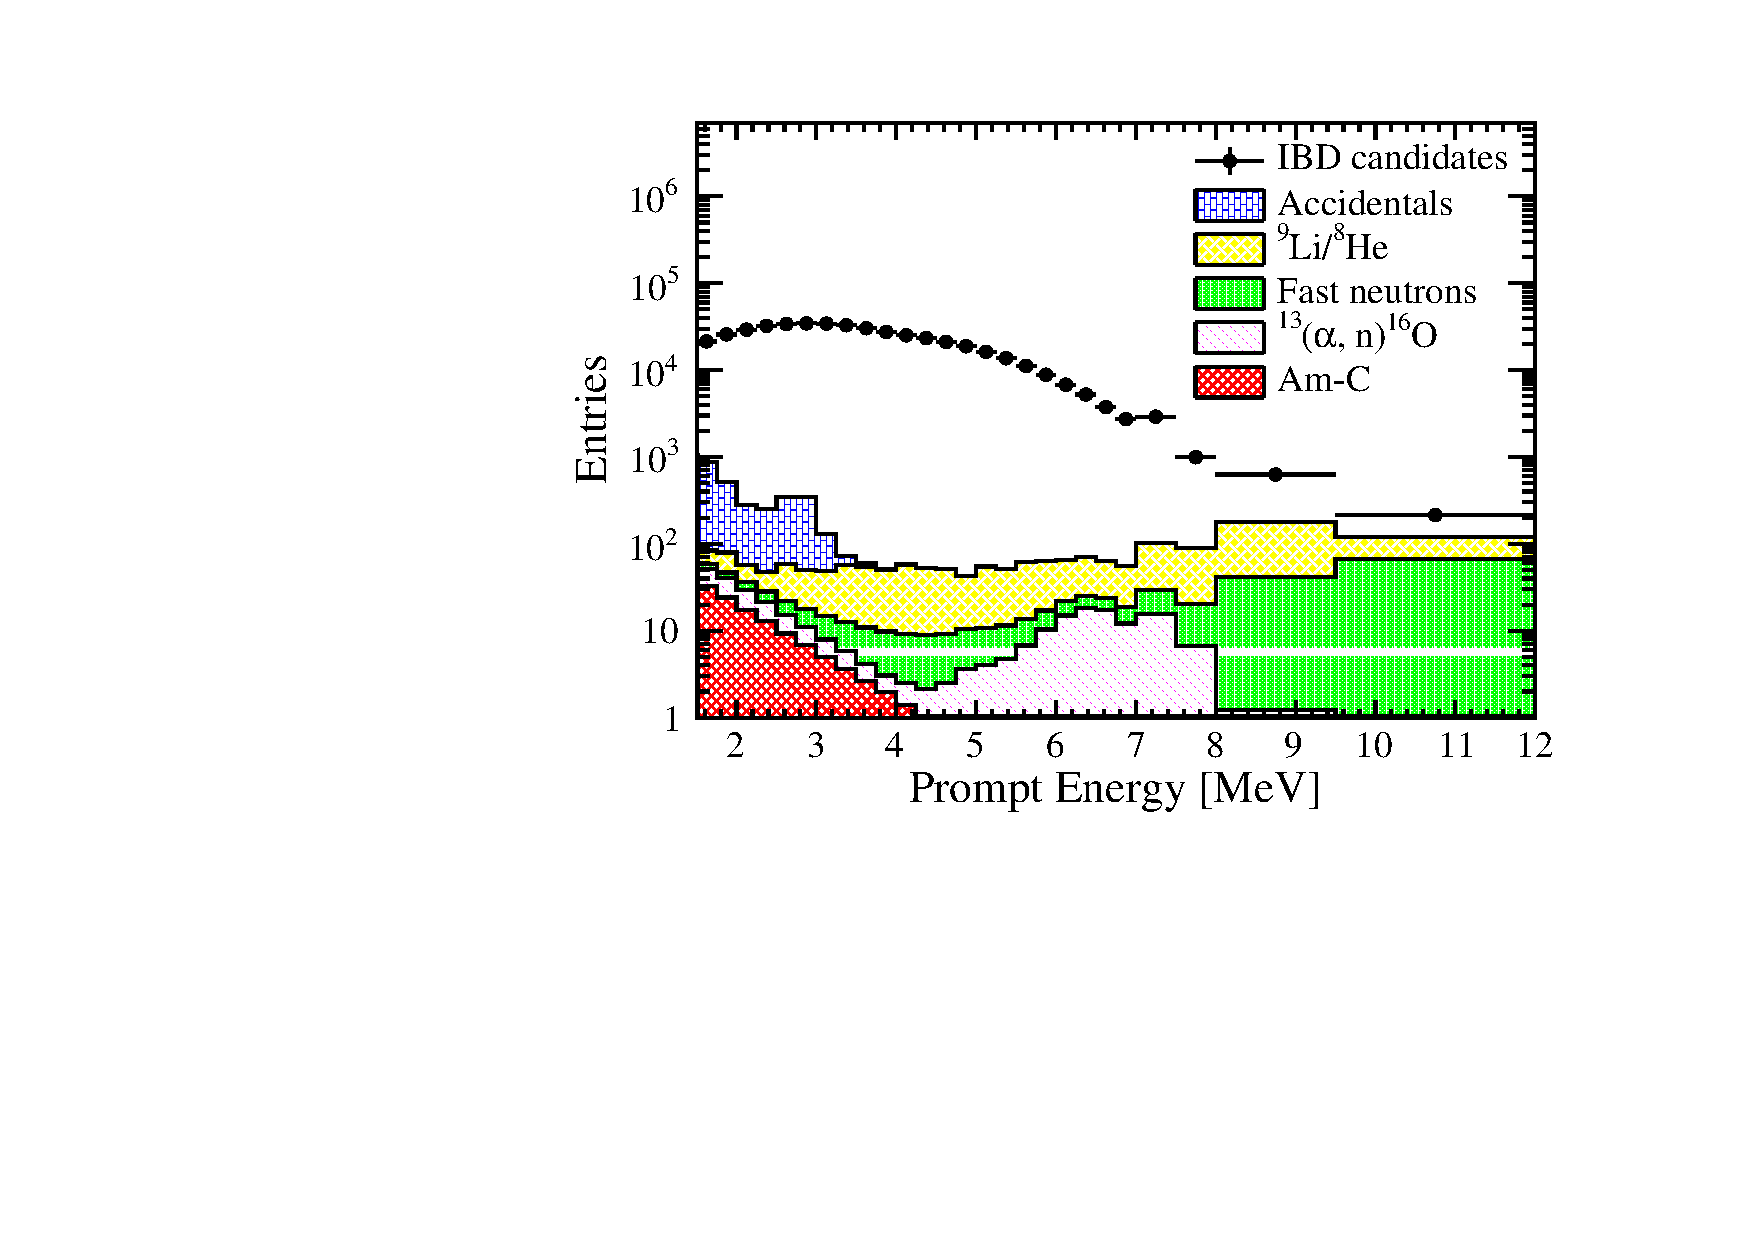
\includegraphics[width=8cm]{nGd-bkg-EH3.pdf}
    \caption*{(b)}
    \end{minipage}
        \caption{(a) 和 (b) 分别是大亚湾1958天数据分析中EH3的$n$H和$n$Gd样本中的信号与本底叠加能谱。}
    \label{fig:nH-nGd-bkgs}
\end{figure}

\subsubsection{系统误差分析与振荡参数拟合}\label{sec:uncertainty}
本项目对$\overline{\nu}_e$的观测结果分为两部分:\qiangdiao{信号事例数和能谱}。振荡参数的拟合也是基于这两项观测结果与理论预期的比较开展的。因此,系统误差是由那些可以影响这两项观测结果的各种因素引入的。

有些系统误差可以影响信号事例数和能谱的观测结果,但由于它们对每个探测器的这种影响都是完全关联的(使每个探测器观测的信号事例数和能谱同比例变化),在大亚湾多个探测器相对测量的策略之下可以忽略。比如热功率等反应堆相关因素和IBD反应截面的系统误差项,它们对每个探测器观测结果的影响都是完全关联的,且在之前的分析中已得到充分研究。

还有一些系统误差项在探测器间是不关联的,但由于其估计策略与具体的数据集无关,不需要在新的数据集中被重复研究。比如每个探测器的质子数的非关联误差,是由实验初期的实地测量结果计算出的。还有一些探测效率,它们需要针对新的数据集进行更新,但由于估计结果精确其误差总被忽略。比如光电倍增管自发光噪声排除效率、宇宙线缪子反符合效率和事例多重数选择效率,其对应的误差可以被忽略。

\paragraph{探测效率的估计及其系统误差}
\qiangdiao{总结而言,本项目中关键的与信号事例数相关的系统误差可归结为以下三项探测效率的系统误差:快信号能量选择效率、慢信号能量选择效率和快慢信号之间距离-时间联合选择效率。}

其中的两项能量选择效率在不同探测器部分差异较大。因此将探测器靶物质按照材料不同分为GdLS、LS、亚克力材料和白油,并将亚克力材料按照几何位置分为内亚克力罐、外亚克力罐和其他亚克力材料这三部分,分别对能量效率展开研究。而距离-时间联合选择效率的研究则可以从数据出发,对整个探测器开展。

快信号能量选择范围对每个探测器都是固定且相同的,其最主要的误差来源是探测器间能标的差异。实验需要根据各种$\alpha$和$\gamma$源比较探测器间的能标差异,进而估计这种能标差异会导致的效率系统误差。

慢信号能量选择范围对八个探测器是各自浮动的,具体是根据它们各自的$n$H信号峰的峰位和分辨率确定的。因此,能标对该项效率的影响较小,但探测器间能够影响谱形的因素均可对其产生影响。比如不同探测器如果具有的死物质几何是不同的,慢信号的能量泄露效应将在探测器间具有差异性,进而会造成2.2 MeV峰位附近的信号占比在不同探测器的差异。

距离和时间的选择范围对每个探测器也是固定且相同的。这意味着那些能使中子的传播与俘获时间在探测器间不同的可能因素都是该项效率系统误差的来源。幸运的是,从数据中可以直接评估这一效率并比较其在探测器间的差异,从而考虑了潜在多种系统误差来源的综合影响。

\paragraph{能谱的预测及其系统误差}
能谱的预测需要建立起中微子能量到IBD快信号观测能量的转换关系。这一转换关系由探测器响应模型决定。该模型依次考虑IBD正电子和中子在探测器中的能量沉积与泄露,液闪发光非线性,电子学非线性,能量分辨率和空间非均匀性的影响。其中,液闪非线性主要是电离淬灭和切伦科夫光导致的,前者可以使高电离密度粒子的光产额降低,比如质子、$\alpha$粒子和低能$e^\pm$,后者则可以在粒子超过液闪中光的相速度的情况下使光产额增加,从而使沉积能量和可见光能量不成正比。电子学非线性则是由于探测到光子的时间分布和电子学读出系统的采集效率对电荷重建结果的影响引发的。利用该模型可以研究上述单一效应的变化对探测效率和能谱的影响。根据现有的分析,起主要贡献的能谱预测系统误差来源包括探测器能标的相对和绝对差异,液闪非线性和电子学非线性,亚克力材料几何的相对差异。

\paragraph{振荡参数的拟合}
振荡参数拟合的基本策略是根据每个探测器每个能量区间下的IBD信号数的观测值与预测值的差异建立$\chi^2$,将$\chi^2$极小化就可以获得振荡参数的最优拟合值。振荡参数$\sin^22\theta_{13}$和$\Delta m_{32}^2$值的变化直接影响$\chi^2$中信号数和能谱的预测结果。系统误差则以惩罚参数的形式引入。每项系统误差对应的惩罚参数以特定方式影响$\chi^2$中预测值的变化,而这些参数的变化程度由其系统误差限制,并贡献到$\chi^2$中。

\subsubsection{$n$H和$n$Gd分析结果的联合}\label{sec:nGdnH-combine}
\qiangdiao{为了完成$n$H和$n$Gd分析结果的联合,关键任务是研究两个分析结果之间的关联系数。}关联性按照来源可以分为:探测效率,IBD能谱,本底和反应堆相关的因素。其中反应堆相关的因素对于两个分析是完全关联的。两个分析虽然具有显著不同靶体积和选择条件,本底的成分也极为不同,但能量测量手段、部分本底分析方法和能量非线性等因素都具有关联性。\qiangdiao{根据之前的分析,基于事例率的$n$H分析结果与$n$Gd分析结果之间的关联系数仅为2\%。} 新的氢俘获分析引入了新的本底:放射性中子本底,还开展了基于能谱的振荡参数测量。这些因素都会改变两个分析的相关性。\qiangdiao{本项目将进一步对基于事例率和能谱测量的$n$H和$n$Gd分析结果之间的关联性进行研究,完成两组振荡参数测量的联合,提高精度。}

\subsection{研究目标}
本项目预期完成以下研究目标。

\paragraph{目标一} 更新宇生本底研究并开展新的muon-x本底研究,使其与快中子本底的联合估计精度达到约20\%,将$^9$Li/$^8$He本底事例率的估计精度从约50\%提升至约30\%;
\paragraph{目标二} 将探测效率的联合系统误差减小约四分之一;
\paragraph{目标三} 将氢俘获研究单独的$\sin^22\theta_{13}$测量精度从7\%提升至6\%,$\Delta m_{32}^2$测量精度从5.6\%提升至约4.8\%。通过联合分析将钆俘获分析的$\sin^22\theta_{13}$测量精度从2.8\%提升到约2.5\%,$\Delta m_{32}^2$的测量精度从2.4\%提升到约2.2\%。

\subsection{拟解决的关键科学问题}
\qiangdiao{本项目将解决两个关键科学问题:A. 使用完整的$n$H样本完成基于事例率和能谱的中微子振荡振幅和频率的同时测量;B. 联合$n$H和$n$Gd分析对振荡参数的测量结果。}

\qiangdiao{A问题在大亚湾实验,RENO实验和Double Chooz实验目前已发表的$n$H分析中都尚未实现。}该问题的困难性在于$n$H样本中的$\overline{\nu}_e$信号主要来自探测器更靠外的纯液闪中,能量泄露效应明显、本底高和系统误差显著等因素都造成其IBD能谱难以估计。立足于本项目的研究条件,这一科学问题的解决具有充分的条件。

\qiangdiao{B问题立足于A问题之上,是大亚湾实验主要物理目标的最终实现,旨在充分利用大亚湾实验相比于其他实验的优势,提供国际上$\theta_{13}$最精确的测量结果,对中微子未知参数的探索具有重要意义。}

\NsfcSection{3}{拟采取的研究方案及可行性分析}{(包括研究方法、技术路线、实验手段、关键技术等说明);}
\subsection{研究方案}

\cref{fig:CalibrationProce}展示了本项目拟议的技术路线图,其中方框表明了重要研究节点对应的分析结果,箭头上的简短说明文字总结为了得到该研究结果所需实现的分析。

本项目从大亚湾实验2011年12月24日至2020年12月12日共运行3158天采集并完成刻度与重建的数据出发,首先使用1500 $\mu$s的符合时间窗和1.5 MeV的低能阈值条件选择出二重符合的快慢信号事例对。对这些事例施加完整的能量和距离-时间选择条件可以得到 \qiangdiao{$\overline{\nu}_e$候选事例样本}。在得到该样本的同时,可以获得事例间不满足符合条件的单事例样本。基于该单事例样本可以精确估计出偶然符合本底的事例率和分布特征。将偶然符合本底从$\overline{\nu}_e$候选样本中扣除就得到了\qiangdiao{关联$\overline{\nu}_e$候选样本}。

\begin{figure}
  \centering
  \resizebox{1.0\textwidth}{!}{
    \begin{tikzpicture}[node distance=5em, text width=5em]
      %定义流程图具体形状+        \small
      \node[startstop](data){大亚湾实验重建数据};
      \node[startstop, right of = data, xshift=3em](candidates){$\overline{\nu}_e$候选事例样本};
      \node[startstop, right of = candidates, xshift = 3em](bkgsub){关联$\overline{\nu}_e$候选样本};
      \node[startstop, right of = bkgsub,xshift = 3em](ADcheck){探测效率及其系统误差};
      \node[startstop, right of = ADcheck,xshift = 3em](shapeuncer){能谱预测及其系统误差};
      \node[startstop, below of = bkgsub](corrbkg){关联本底};
      \node[startstop, below of = shapeuncer](nHresult){$n$H样本振荡分析结果};
      \node[startstop, below of = nHresult](combine){$n$H和$n$Gd结果合并};
      %连接具体形状
      % \draw (dec1) -- node [above] {N} (point1);
      \draw [arrow] (data)  -- node [above, yshift=1.3em] {时间符合} (candidates);
      \draw [arrow] (candidates)  -- node [above, yshift=1.3em, text width=5em,align=center] {扣除偶然符合本底} (bkgsub);
      \draw [arrow] (bkgsub)  -- node [above, yshift=1.3em, text width=8em,align=center] {探测器一致性检查和模拟数据研究} (ADcheck);
      \draw [arrow] (bkgsub)  -- node [left, text width=14em, yshift=-0.5em, align=center] {宇生本底和放射性中子本底估计} (corrbkg);
      \draw [arrow] (corrbkg)  -- node [above, yshift=0.2em, text width=5em,align=center] {建立$\chi^2$} (nHresult);
      \draw [arrow] (ADcheck)  -- node [above, yshift=1.3em, text width=5em,align=center] {能量响应模型} (shapeuncer);
      \draw [arrow] (shapeuncer)  -- node [above, yshift=-0.65em, text width=5em,align=center] {} (nHresult);
      \draw [arrow] (nHresult)  -- node [left, xshift=1.45em, yshift=-0.2em, text width=15em,align=center] {$n$H与$n$Gd研究结果的关联性分析} (combine);
    \end{tikzpicture}
  }
  \caption{本项目拟议的技术路线图。方框中的文字描述了重要节点对应的研究结果,箭头上的文字说明了关键技术。}
  \label{fig:CalibrationProce}
\end{figure}

关联$\overline{\nu}_e$候选样本中的本底占比极少,可以基于该样本开展探测器一致性检查。检查的重点是八个探测器的能标、分辨率、信号能谱和距离时间联合分布的差异。结合这些差异与模拟样本的研究可以估计出\qiangdiao{探测效率及其系统误差}。使用新的探测器非线性数据更新现有的能量响应模型,并\qiangdiao{预测信号能谱},进一步联合这些探测器差异与该模型就可以估计出各项探测器相关的因素可能\qiangdiao{对能谱导致的系统误差}。这就完成了信号数与能谱的预测以及它们的系统误差研究。

根据$\overline{\nu}_e$候选样本中的事例与缪子事例的关联性,可以估计出其中各项宇生本底的贡献。根据探测器材料的放射性含量测量结果与理论计算,可以估计出放射性中子本底的贡献。结合之前数据研究中的刻度源本底分析结果,能够以线性关系推算出新数据中的Am-C刻度源本底的贡献。这就完成了信号样本中的\qiangdiao{关联本底分析}。其中,以数据驱动的方法验证放射性中子本底的理论估计结果是一个可能的改进点。

基于信号样本和本底评估的统计结果,与信号事例数和能谱的预测结果建立$\chi^2$,并以惩罚参数的形式考虑进探测效率和能谱的系统误差项的影响,然后保持振荡参数$\sin^22\theta_{13}$和$\Delta m_{32}^2$为自由参数将$\chi^2$极小化,就得到了\qiangdiao{$n$H-IBD样本的振荡分析结果}。改变拟合中的数据筛选条件可以对该分析结果进行检验。

$n$Gd-IBD样本的研究结果已经公布。逐项基于物理来源和估计方法分析$n$H与$n$Gd分析中每个系统误差项的关联性,并将其合并以得到总体上两个分析结果的相关系数,就可以\qiangdiao{对两项振荡参数拟合结果进行联合}。

在1958天的$n$H样本分析中,\qiangdiao{$\theta_{13}$最主要的误差来源是统计误差与探测效率的系统误差},这两项的贡献基本相同。统计误差通过使用完整的$n$H样本可以得到显著压低。探测效率的系统误差来源主要是快慢信号能量的选择和距离时间联合选择。慢信号能量的选择效率与距离时间联合选择效率,这两项的系统误差评估都是基于真实数据样本开展的,会受到统计量的限制,因此也会在大统计量样本研究中得到改善。而快信号能量选择效率的系统误差最主要的来源是探测器间能标的相对差异,这在之前的分析中被评估为0.5\%,明显大于$n$Gd分析中的0.2\%。因此在本项目的研究中,能量,特别是能标的系统误差将会是一个研究重点和难点。
据此,上述路线图中可能的难点与预期解决方案如下。
\paragraph{\qiangdiao{难点一:$^9$Li/$^8$He样本时间谱的拟合。}}对$^9$Li/$^8$He本底事例率的评估精度提升的预期可能因统计量和信噪比的限制受限。本项目计划参考$n$Gd分析,将$^9$Li/$^8$He本底样本的快信号能量筛选条件从3.5 MeV提升至8 MeV,以提高$^9$Li/$^8$He在该样本中的信噪比,从而提高估计的精度。但提高能量阈值后,整体样本的统计量会下降。$^9$Li/$^8$He含量的估计是通过拟合事例相距缪子的时间分布,需要改进该拟合的鲁棒性才能给出估计结果。预期,灵活调整$^9$Li/$^8$He能量阈值以平衡统计量与信噪比的关系,并优化时间谱拟合的条件,可以妥善解决此问题。
\paragraph{\qiangdiao{难点二:探测器一致性检验时样本的选择与修正。}}在评估系统误差时需要比较和理解不同样本呈现出的探测器一致性的差异,并可能需要对非IBD样本的研究结果进行修正。比如,研究能标和能谱在探测器间的差异会着重参考IBD样本和散裂中子样本呈现的结果,这是因为两个样本的高度相似性。但是后者与宇宙线有关,在三个实验厅的具体性质存在差异,这一特性对探测器差异研究结果的影响需要仔细考虑。除此之外,为了降低能量相关的系统误差,需要对这两个样本之外的一致性结果进行检验。再比如,比较距离时间联合分布在探测器间的差异时会着重参考IBD样本和$^{214}$Bi-$^{214}$Po样本,也是因为两个样本的相似性。但对于二者不同之处可能需要修正,而修正可能存在一定困难。因为IBD样本主要分布在LS区间,$^{214}$Bi-$^{214}$Po样本虽在LS区间也有分布但主要还是集中在GdLS区域。按照探测器不同区域将$^{214}$Bi-$^{214}$Po样本的距离时间分布按照IBD样本进行归一化修正时,LS边界处的$^{214}$Bi-$^{214}$Po过低的统计量会影响修正效果。预期,结合完整数据更大的统计量,尝试多种修正方法和使用多种参考样本给出一致的系统误差评估结果,能够解决这一问题。
 \paragraph{\qiangdiao{难点三:基于能谱拟合的关联性分析。}}根据$n$Gd和$n$H分析的各项系统误差的关联性导出两个结果整体关联性时,与能谱相关的关联性需要额外考量。在之前基于事例率的分析中,只有探测效率和本底估计会影响信号事例数,而反应堆相关的项对两个分析是完全关联的。在本项目的基于事例率和能谱的分析中,振荡参数$\sin^22\theta_{13}$和$\Delta m_{32}^2$的拟合将利用八个探测器在不同能量点处的统计信息。而$n$H-IBD和$n$Gd-IBD的能谱的关联性是复杂的,比如与反应堆相关的项、能量非线性和能标等因素都是关联的,而能量泄露和非均匀性等效应又是不关联的。预期,如果根据两个分析每一项的关联系数难以估计整体结果的关联系数,可以考虑联合两个分析的$\chi^2$进行拟合,可以使这一问题得到妥善解决。

\subsection{可行性分析}
\qiangdiao{对$\theta_{13}$的测量是大亚湾中微子实验的主要物理目标。基于大亚湾实验完整数据集的整理情况与以往数据集的中微子振荡研究成果,本项目的可行性具有充分的依据。}

大亚湾完整数据集已完成刻度与重建,使用该批数据的钆俘获样本振荡研究结果整理的文章已经提交到\texttt{arxiv.org}网站。有两篇基于以往大亚湾数据的$n$H样本的振荡研究文章经过了合作组内部的严格审查,已经发表到Physical Review D期刊上。目前,基于1958天$n$H样本的研究在大亚湾合作组内已经完成并完成分析工作的评审,即将开始论文评审。在合作组内部的多次讨论下,预期这一成果将于近期发表在Physical Review Letter期刊上。这些论文和研究给本项目的研究内容提供了切实具体的可参考信息。基于完整$n$H样本的研究难点及其解决方案在本项目中都已被讨论。通过这些信息可以看出,本项目具有坚实可靠的可行性。

\NsfcSection{4}{本项目的特色与创新之处;}{}

本项目的特色和创新之处在于将克服基于$n$H样本振荡分析的诸多难点,利用大亚湾反应堆中微子实验的完整$n$H样本同时给出中微子振荡振幅和频率的测量,\qiangdiao{基于单一$n$H样本提供国际上第二精确的$\theta_{13}$测量值},进一步将其与$n$Gd分析结果联合将\qiangdiao{提供国际上最精确$\theta_{13}$测量值}和与加速器实验同等精度的$\Delta m_{32}^2$测量值,对未来中微子物理未知的基本参数的探索具有重要价值。

\NsfcSection{5}{年度研究计划及预期研究结果}{(包括拟组织的重要学术交流活动、国际合作与交流计划等)。}

项目的研究计划为:
\begin{itemize}
	\item 2024年1月1日-2024年12月31日:基于氢俘获样本完成中微子振荡参数$\theta_{13}$和$\Delta m_{32}^2$的测量;
	\item 2025年1月1日-2025年12月31日:对氢俘获样本研究结果进行交叉检验,完成氢俘获样本和钆俘获研究的关联性分析,开展$n$H和$n$Gd研究的$\theta_{13}$与$\Delta m_{32}^2$测量结果的合并;
	\item 2026年1月1日-2026年12月31日:总结研究成果,在大亚湾实验合作组内部完成研究工作的评审、论文评审,将论文发表至期刊上。
\end{itemize}

项目研究期间,本项目申请人将与合作组内的国际研究者展开多方合作,将在大亚湾国际合作组组会多次报道研究进展,取得关键成果并发表后将在一系列重要国际会议如NEUTRINO,国际高能物理大会(ICHEP)和欧洲物理学会高能物理会议(EPS-HEP),包括中国物理学会高能物理会议上报道研究结果。

\qiangdiao{预期本项目将给出国际上最精确的混合角$\theta_{13}$测量结果和与加速器实验同等精度的$\Delta m_{32}^2$测量结果。单一氢俘获样本的研究的测量精度预计约6\%,$n$H和$n$Gd样本的联合研究研究将会使目前$n$Gd样本的测量精度从2.8\%提升至约2.5\%。}本项目的研究成果将总结为一篇详细的研究文档在实验合作组内存档,并发表两篇期刊文章,包括一篇阐述研究细节的Physical Review D长文章和一篇报道关键结果的Physical Review Letter短文章。

\NsfcChapter{(二)研究基础与工作条件}{}

\NsfcSection{1}{研究基础}{(与本项目相关的研究工作积累和已取得的研究工作成绩);}

本项目课题组在大亚湾氢俘获样本的振荡分析工作上具有深厚的积累。大亚湾实验在2014年和2016年基于氢俘获数据集发表的$\theta_{13}$测量结果:\qiangdiao{\texttt{Phys. Rev. D 90, 071101 (2014)}}和\qiangdiao{\texttt{Phys. Rev. D 93, 072011 (2016)}},都是由本项目课题组在合作组内主导完成的。本项目课题组还曾独立承担\qiangdiao{科技部国家重点研发计划在大科学装置前沿研究专项下的《氢俘获中微子振荡研究》子课题}。本项目申请人以主要参与者的身份支撑了该项课题的验收工作,并在2022年以此为基础完成了\qiangdiao{题为《在大亚湾用氢俘获法研究中微子振荡频率和振幅》的博士学位论文}。该学位论文的研究基于大亚湾1958天的氢俘获数据实现了$\sin^22\theta_{13}$和$\Delta m_{32}^2$的同时测量。 

\NsfcSection{2}{工作条件}{(包括已具备的实验条件,尚缺少的实验条件和拟解决的途径,包括利用国家实验室、国家重点实验室和部门重点实验室等研究基地的计划与落实情况);}

本项目课题组包含多位教授和研究员。这些成员参与了国际上多个中微子实验组的研究,比如大亚湾和Super-K实验,具有中微子振荡实验的丰富经验。此外,由于以往相关基金的支持和合作组的支持,本项目组完全具备了相关的研究和工作条件。

\NsfcSection{3}{正在承担的与本项目相关的科研项目情况}{(申请人正在承担的与本项目相关的科研项目情况,包括国家自然科学基金的项目和国家其他科技计划项目,要注明项目的资助机构、项目类别、批准号、项目名称、获资助金额、起止年月、与本项目的关系及负责的内容等);}

无。

\NsfcSection{4}{完成国家自然科学基金项目情况}{(对申请人负责的前一个已资助期满的科学基金项目(项目名称及批准号)完成情况、后续研究进展及与本申请项目的关系加以详细说明。另附该项目的研究工作总结摘要(限500字)和相关成果详细目录)。}

无。

\NsfcChapter{(三)其他需要说明的情况}{}

\NsfcSection{1}{}{申请人同年申请不同类型的国家自然科学基金项目情况(列明同年申请的其他项目的项目类型、项目名称信息,并说明与本项目之间的区别与联系)。}

无。

\NsfcSection{2}{}{具有高级专业技术职务(职称)的申请人是否存在同年申请或者参与申请国家自然科学基金项目的单位不一致的情况;如存在上述情况,列明所涉及人员的姓名,申请或参与申请的其他项目的项目类型、项目名称、单位名称、上述人员在该项目中是申请人还是参与者,并说明单位不一致原因。}

无。

\NsfcSection{3}{}{具有高级专业技术职务(职称)的申请人是否存在与正在承担的国家自然科学基金项目的单位不一致的情况;如存在上述情况,列明所涉及人员的姓名,正在承担项目的批准号、项目类型、项目名称、单位名称、起止年月,并说明单位不一致原因。}

无。

\NsfcSection{4}{}{其他。}

无。

\end{document}
